\section{Discretization}
\subsection{Options}
The 3 options are zero-order hold, Euler's rule and the bilinear transformation. (using a sampling time of $T_s=0.05s$). The matrix A is not invertible which means that the zero and hold is not feasible. 

\subsection{Choice of discretization rule}
The bilinear transformation always maps stable poles in the continuous domain to stable poles in the discrete domain. However in this particular case both Euler and the bilinear transformation have stable poles. 

Both the bilinear and Euler are fully controllable and observable.(and so also detectable and stabilisable) The only real difference is in the transmission zeros, the  bilinear transformation has transmission zeros while Euler does not. And thats why the  bilinear transformation is the preferred choice in this case. As transmission zeros are stable which means the system is minimum phase system as the 8 transmission zeros are all -1 which is inside the unit circle. There is also the argument that the bilinear transformation maps the zeros over the entire unit circle, while the backward rectangle method does not. This makes the bilinear transformation the most elegant one.

The mathematical formulas for the bilinear transformation:
$$A_d= \left(I -  \frac{AT_s}{2}\right)^{-1} \left(I+\frac{AT_s}{2}\right)$$
$$B_d=\left(I -  \frac{AT_s}{2}\right)^{-1} B T_s$$
$$C_d=C\left(I -  \frac{AT_s}{2}\right)^{-1}$$
$$D_d=D+C\left(I -  \frac{AT_s}{2}\right)^{-1}\frac{BT_s}{2}$$


\subsection{Properties discrete model}
\subsubsection{Zeros and poles}
Figure~\ref{fig:zplot_disc} contains the poles and zeros of the discrete system. There are 8 transmission zeros all at -1. The poles are all near 1, with 8 of them on 1 and 4 of them at about 0.9753. As all the poles are within the unit circle the system is stable
\begin{figure}[H]
	\centering
	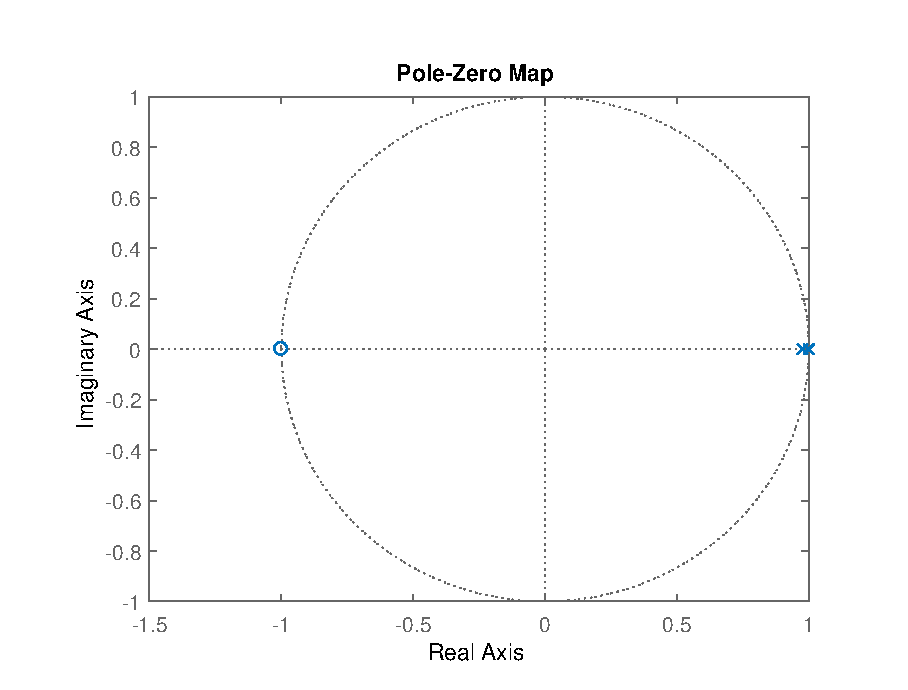
\includegraphics[width=7cm]{./img/discrete/zplot.eps}
	\caption{zplot of the new discrete system}
	\label{fig:zplot_disc}
\end{figure}

\subsubsection{Observability and controllability} 
the rank of the controllability matrix is 12 with the smallest singular value being $2.099 \cdot 10^{-3}$. The rank of the observability matrix is 12, with the smallest singular value being 4.213 $\cdot 10^{-1}$. If there where singular values in the neighborhood of the machine precision $10^{-15}$ this would imply the the matrices might just be of full rank due to numerical errors. Which would make the system potentially not controllable/observable.

\subsubsection{Detectable Stabilisable}
As the system is observable this means that the system is also detectable, And as the system is controllable it is stabilisable. 

\subsubsection{Is the system minimum}
The system is minimum, often times a system that is not minimum will not be fully observable or controllable. So its important to have the minimum realization.

\subsection{Numerical values matrices}
$$
A_{discrete}=
\begin{bmatrix}
1.0000&0&0&0.0494&0&0&0&0.0121&0&0&0.0003&0 \\
0&1.0000&0&0&0.0494&0&-0.0121&0&0&-0.0003&0&0 \\
0&0&1.0000&0&0&0.0494&0&0&0&0&0&0 \\
0&0&0&0.9753&0&0&0&0.4844&0&0&0.0121&0 \\
0&0&0&0&0.9753&0&-0.4844&0&0&-0.0121&0&0 \\
0&0&0&0&0&0.9753&0&0&0&0&0&0 \\
0&0&0&0&0&0&1.0000&0&0&0.0500&0&0 \\
0&0&0&0&0&0&0&1.0000&0&0&0.0500&0 \\
0&0&0&0&0&0&0&0&1.0000&0&0&0.0500 \\
0&0&0&0&0&0&0&0&0&1.0000&0&0 \\
0&0&0&0&0&0&0&0&0&0&1.0000&0 \\
0&0&0&0&0&0&0&0&0&0&0&1.0000 \\
\end{bmatrix}
$$

$$
B_{discrete}=
\begin{bmatrix}
0&0&0&0 \\
0&0&0&0 \\
10^{-4}&10^{-4}&10^{-4}&10^{-4} \\
0&10^{-4}&0&-5\cdot 10^{-4} \\
-5 \cdot 10^{-4}&0&5 \cdot 10^{-4}&0 \\
3\cdot 10^{-3}&3\cdot 10^{-3}&3\cdot 10^{-3}&3\cdot 10^{-3} \\
1.9\cdot 10^{-3}&0&-1.9\cdot 10^{-3}&0 \\
0&1.9\cdot 10^{-3}&0&-1.9\cdot 10^{-3} \\
1.3 \cdot 10^{-3}&-1.3 \cdot 10^{-3} &1.3 \cdot 10^{-3}&-1.3 \cdot 10^{-3} \\
7.5\cdot 10^{-2}&0&-7.5\cdot 10^{-2}&0 \\
0&7.5\cdot 10^{-2}&0&-7.5\cdot 10^{-2} \\
5\cdot 10^{-2}&-5\cdot 10^{-2}&5\cdot 10^{-2}&-5\cdot 10^{-2} \\
\end{bmatrix}
$$

$$
C_{discrete}=
\begin{bmatrix}
1&0&0&0.0247&0&0&0&0.0061&0&0&0.0002&0 \\
0&1&0&0&0.0247&0&-0.0061&0&0&-0.0002&0&0 \\
0&0&1&0&0&0.0247&0&0&0&0&0&0 \\
0&0&0&0&0&0&1&0&0&0.0250&0&0 \\
0&0&0&0&0&0&0&1&0&0&0.0250&0 \\
0&0&0&0&0&0&0&0&1&0&0&0.0250 \\
\end{bmatrix}
$$

$$
D_{discrete}=
10^{-3} \cdot
\begin{bmatrix}
0&0.0057&0&-0.0057 \\
-0.0057&0&0.0057&0 \\
0.0370&0.0370&0.0370&0.0370 \\
0.9375&0&-0.9375&0 \\
0&0.9375&0&-0.9375 \\
0.6250&-0.6250&0.6250&-0.6250 \\
\end{bmatrix}
$$